\documentclass[a4paper,14pt]{extreport}
\usepackage[left=1.5cm,right=1.5cm,
    top=1.5cm,bottom=2cm,bindingoffset=0cm]{geometry}
\usepackage{scrextend}
\usepackage[T1,T2A]{fontenc}
\usepackage[utf8]{inputenc}
\usepackage[english,russian,ukrainian]{babel}
\usepackage{tabularx}
\usepackage{amssymb}
\usepackage{color}
\usepackage{amsmath}
\usepackage{mathrsfs}
\usepackage{listings}
\usepackage{graphicx}
\graphicspath{ {./images/} }
\usepackage{lipsum}
\usepackage{xcolor}
\usepackage{hyperref}
\usepackage{tcolorbox}
\usepackage{tikz}
\usepackage[framemethod=TikZ]{mdframed}
\usepackage{wrapfig,boxedminipage,lipsum}
\mdfdefinestyle{MyFrame}{%
linecolor=blue,outerlinewidth=2pt,roundcorner=20pt,innertopmargin=\baselineskip,innerbottommargin=\baselineskip,innerrightmargin=20pt,innerleftmargin=20pt,backgroundcolor=gray!50!white}
 \usepackage{csvsimple}
 \usepackage{supertabular}
\usepackage{pdflscape}
\usepackage{fancyvrb}
%\usepackage{comment}
\usepackage{array,tabularx}
\usepackage{colortbl}

\usepackage{varwidth}
\tcbuselibrary{skins}
\usepackage{fancybox}
\usepackage{multicol}
\usepackage{multirow}


\usepackage{tikz}
\usepackage[framemethod=TikZ]{mdframed}
\usepackage{xcolor}
\usetikzlibrary{calc}
\makeatletter
\newlength{\mylength}
\xdef\CircleFactor{1.1}
\setlength\mylength{\dimexpr\f@size pt}
\newsavebox{\mybox}
\newcommand*\circled[2][draw=blue]{\savebox\mybox{\vbox{\vphantom{WL1/}#1}}\setlength\mylength{\dimexpr\CircleFactor\dimexpr\ht\mybox+\dp\mybox\relax\relax}\tikzset{mystyle/.style={circle,#1,minimum height={\mylength}}}
\tikz[baseline=(char.base)]
\node[mystyle] (char) {#2};}
\makeatother

\definecolor{ggreen}{rgb}{0.4,1,0}
\definecolor{rred}{rgb}{1,0.1,0.1}
\definecolor{amber}{rgb}{1.0, 0.75, 0.0}
\definecolor{babyblue}{rgb}{0.54, 0.81, 0.94}
\definecolor{amethyst}{rgb}{0.6, 0.4, 0.8}

\usepackage{float}
\usepackage{wrapfig}
\usepackage{framed}
%for nice Code{
\lstdefinestyle{customc}{
  belowcaptionskip=1\baselineskip,
  breaklines=true,
  frame=L,
  xleftmargin=\parindent,
  language=C,
  showstringspaces=false,
  basicstyle=\small\ttfamily,
  keywordstyle=\bfseries\color{green!40!black},
  commentstyle=\itshape\color{purple!40!black},
  identifierstyle=\color{blue},
  stringstyle=\color{orange},
}
\lstset{escapechar=@,style=customc}
%}


\begin{document}
\pagecolor{white}

%----------------------------------------1
\newtcbox{\xmybox}[1][red]{on line, arc=7pt,colback=#1!10!white,colframe=#1!50!black, before upper={\rule[-3pt]{0pt}{10pt}},boxrule=1pt, boxsep=0pt,left=6pt,right=6pt,top=2pt,bottom=2pt}

\begin{titlepage}
  \begin{center}
    \large
    Національний технічний університет України \\ "Київський політехнічний інститут імені Ігоря Сікорського"


    Факультет Електроніки

    Кафедра мікроелектроніки
    \vfill

    \textsc{ЗВІТ}\\

    {\Large Про виконання лабораторної роботи №3\\
      з дисципліни: «Схемотехніка-1»\\[1cm]

        ОПЕРАЦІЙНІ ЛАНКИ НУЛЬОВОГО ПОРЯДКУ


    }
  \bigskip
\end{center}
\vfill

\newlength{\ML}
\settowidth{\ML}{«\underline{\hspace{0.4cm}}» \underline{\hspace{2cm}}}
\hfill
\begin{minipage}{1\textwidth}
Виконавець:\\
Студент 3-го курсу \hspace{4cm} $\underset{\text{(підпис)}}{\underline{\hspace{0.2\textwidth}}}$  \hspace{1cm}А.\,С.~Мнацаканов\\
\vspace{1cm}

Перевірила: \hspace{6.1cm} $\underset{\text{(підпис)}}{\underline{\hspace{0.2\textwidth}}}$  \hspace{1cm}Г.\,С.~Порева\\

\end{minipage}

\vfill

\begin{center}
2021
\end{center}
\end{titlepage}


\begin{center}Мета роботи\end{center}\par
Вивчення принципів роботи, дослідження амплітудних
характеристик та параметрів різних функціональних ланок на основі
інтегральних операційних підсилювачів (інвертуючого та неінвертуючого
підсилювачів, сумуючого та віднімаючого підсилювачів).

\begin{figure}[h]
\center{\includegraphics[width=0.8\linewidth]{s.png}}
\caption{Блок-схема лабораторного макета «Операційні ланки нульового
порядку».}
\end{figure}\par

Лабораторна установка для дослідження лабораторного модуля
«ОЛНП» складається з генератора гармонічних коливань 1 типу Г3-112,
лабораторного стенду 2 типу «Каскад М», вольтметрів 3 і 5 типу В3-38,
осцилографа 4 типи С1-55. До складу лабораторного стенду 2 входять
стабілізований блок живлення, електронний комутатор, формувач
імпульсів, чотири лабораторних модулі.\\

Генератор 1 є джерелом гармонійного вихідної напруги в частотному
діапазоні від 20 Гц до 1 МГц і амплітудою від 0 до 6,3 В.
Вольтметри 3 і 5 призначені для вимірювання амплітуди відповідно
вхідної U 1 та вихідної U 2 напруги від 0,1 мВ до 200 В у діапазоні частот від
20 Гц до 3 МГц.\\

Осцилограф 4 використовується для спостереження на екрані
електронно-променевої трубки форми напруги та виміру параметрів
напруги від 30 мВ до 140 В в частотному діапазоні від 3 Гц до 10 МГц.
Лабораторний стенд 2 забезпечує включення одного з чотирьох
лабораторних модулів та підключення джерел живлення і джерел змінної
напруги.\\
\newpage


%\begin{figure}[h]
%\center{\includegraphics[width=0.8\linewidth]{op.png}}
%\caption{ІМП}
%\end{figure}


\begin{figure}[h]
\center{\includegraphics[width=0.8\linewidth]{11111.png}}
\end{figure}

\begin{figure}[h]
\center{\includegraphics[width=0.8\linewidth]{123.png}}
\end{figure}

%\begin{figure}[h]
%\center{\includegraphics[width=0.8\linewidth]{op1.png}}
%\caption{НМП}
%\end{figure}
\clearpage




\begin{center}Результати вимiрювань\end{center}\par


\begin{center}
Табл.1. Для вимірювань функцій масштабних підсилювачів (ІМП, НМП).\\[0.5cm]
\begin{tabular}{|c|c|c|c|}
\hline
\multicolumn{1}{|c|}{\multirow{2}{*}{№}} & \multirow{2}{*}{\begin{tabular}[c]{@{}l@{}}Показники роботи\\ підсилювача\end{tabular}}                    & \multicolumn{2}{c|}{\begin{tabular}[c]{@{}c@{}}Підсилювач в\\ схемі\end{tabular}}                                                                 \\ \cline{3-4} 
\multicolumn{1}{|c|}{}                   &                                                                                                            & \multicolumn{1}{c|}{\begin{tabular}[c]{@{}c@{}}ІМП\\ (П1)\end{tabular}} & \multicolumn{1}{c|}{\begin{tabular}[c]{@{}c@{}}НМП\\ (П2)\end{tabular}} \\ \hline
1                                        & \begin{tabular}[c]{@{}l@{}}При $R_1=0$\\ (П6-замкнутий) $U_{\text{г}}$,мВ\end{tabular}                     & 100                                                                     & 100                                                                     \\ \hline
2                                        & \begin{tabular}[c]{@{}l@{}}При $R_1=1$ кОм\\ (П6-розімкнений)\\ $U_1$, мВ\end{tabular}                     & 91,3                                                                    & 99,4                                                                    \\ \hline
3                                        & $R_{\text{вх}}=R_1\dfrac{U_1}{U_{\text{г}}-U_1}$  кОм                                                          & 10,5                                                                 & 165,7                                                                \\ \hline
4                                        & \begin{tabular}[c]{@{}l@{}}При $R_4=\infty$,\\ $U_{2xx}$, мВ\end{tabular}                                  & 199                                                                     & 300                                                                     \\ \hline
5                                        & \begin{tabular}[c]{@{}l@{}}При $R_4=2$ кОм,\\ $U_2$, мВ\end{tabular}                                       & 199                                                                     & 300                                                                     \\ \hline
6                                        & $R_{\text{вих}}=R_4\dfrac{U_{2xx}-U_2}{U_2}$, Ом                                                           & 0                                                                       & 0                                                                       \\ \hline
7                                        & $K_U=\dfrac{U_2}{U_1}$                                                                                     & 2,18                                                                  & 3,018                                                                  \\ \hline
8                                        & $K_I=K_U\dfrac{R_{\text{вх}}}{R_4}$                                                                        & 11                                                                 & 250                                                                \\ \hline
9                                        & $K_P=K_U\cdot{K_I}$                                                                                        & 25                                                                 & 755                                                                \\ \hline
10                                       & Епюри напруги $U_1$(---) та $U_2$(....)                                                                    & протифазні                                                             & синфазні                                                               \\ \hline
11                                       & \begin{tabular}[c]{@{}l@{}}$f_{\text{в}}=f_{max}$, кГц \\ при $U_{2\text{B}}=0,707\cdot{U_2}$\end{tabular} & 500-600                                                                 & 500-600                                                                 \\ \hline
\end{tabular}
\end{center}

\vspace{2cm}
\begin{center}
Табл.2. Для вимірювань амплітудної характеристики неінвертуючого масштабного підсилювача.\\[0.5cm]
\begin{tabular}{|c|c|c|c|c|c|c|}
\hline
Um1, В & 0,0186 & 0,092 & 0,174 & 0,552 & 0,92 & 1,22 \\ \hline
Um2, В & 0,0561 & 0,283 & 0,568 & 1,68  & 2,78 & 3,66 \\ \hline
\end{tabular}
\end{center}
\newpage


\begin{center}
 Розрахунки
\end{center}
\begin{enumerate}
\item Розрахунок вхідного попору ($R_1=1$ кОм)

\begin{enumerate}
\item Підсилювач в схемі ІМП:
\begin{center}
$R_{\text{вх}}=R_1\dfrac{U_1}{U_{\text{г}}-U_1}=10^3\cdot{\dfrac{91,3\cdot{10^{-3}}}{100\cdot{10^{-3}}-91,3\cdot{10^{-3}}}}=10,49$ кОм\\[1cm]
\end{center}

\item Підсилювач в схемі НМП:
\begin{center}
$R_{\text{вх}}=R_1\dfrac{U_1}{U_{\text{г}}-U_1}=10^3\cdot{\dfrac{99,4\cdot{10^{-3}}}{100\cdot{10^{-3}}-99,4\cdot{10^{-3}}}}=165,7$ кОм
\end{center}
\end{enumerate}


\item Розрахунок вихідного попору ($R_4=2$ кОм)

\begin{enumerate}
\item Підсилювач в схемі ІМП:
\begin{center}
$R_{\text{вих}}=R_4\dfrac{U_{2xx}-U_2}{U_2}=2\cdot{10^3} \cdot{\dfrac{199\cdot{10^{-3}}-199\cdot{10^{-3}}}{199\cdot{10^{-3}}}}=0$ Ом\\[1cm]
\end{center}

\item Підсилювач в схемі НМП:
\begin{center}
$R_{\text{вих}}=R_4\dfrac{U_{2xx}-U_2}{U_2}=2\cdot{10^3} \cdot{\dfrac{300\cdot{10^{-3}}-300\cdot{10^{-3}}}{300\cdot{10^{-3}}}}=0$ Ом
\end{center}
\end{enumerate}


\item Розрахунок коефіцієнта передачі напруги

\begin{enumerate}
\item Підсилювач в схемі ІМП:
\begin{center}
$K_U=\dfrac{U_2}{U_1} = \dfrac{199\cdot{10^{-3}}}{91,3\cdot{10^{-3}}}=2,18$\\[1cm]
\end{center}

\item Підсилювач в схемі НМП:
\begin{center}
$K_U=\dfrac{U_2}{U_1} = \dfrac{300\cdot{10^{-3}}}{99,4\cdot{10^{-3}}}=3,018$
\end{center}
\end{enumerate}



\item Розрахунок коефіцієнта передачі струму

\begin{enumerate}
\item Підсилювач в схемі ІМП:
\begin{center}
$K_I=K_U\cdot{\dfrac{R_{\text{вх}}}{R_4}}=2,18\cdot{\dfrac{10,49\cdot{10^3}}{2\cdot{10^3}}}=11$\\
\end{center}

\item Підсилювач в схемі НМП:
\begin{center}
$K_I=K_U\cdot{\dfrac{R_{\text{вх}}}{R_4}}=3,018\cdot{\dfrac{165,7\cdot{10^3}}{2\cdot{10^3}}}=250$
\end{center}
\end{enumerate}



\item Розрахунок коефіцієнта передачі потужності

\begin{enumerate}
\item Підсилювач в схемі ІМП:
\begin{center}
$K_P=K_U\cdot{K_I}=2,18\cdot{11,434}=25$\\
\end{center}

\item Підсилювач в схемі НМП:
\begin{center}
$K_P=K_U\cdot{K_I}=3,018\cdot{250,041}=755$
\end{center}
\end{enumerate}
\end{enumerate}















\newpage
\begin{center}Графіки\end{center}\par

\begin{figure}[h]
\begin{minipage}[h]{0.49\linewidth}
\center{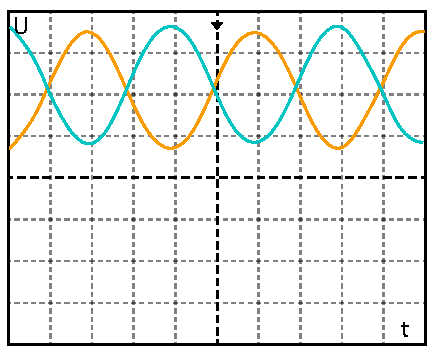
\includegraphics[width=0.9\linewidth]{3.pdf} \\ ІМП}
\end{minipage}
\hfill
\begin{minipage}[h]{0.49\linewidth}
\center{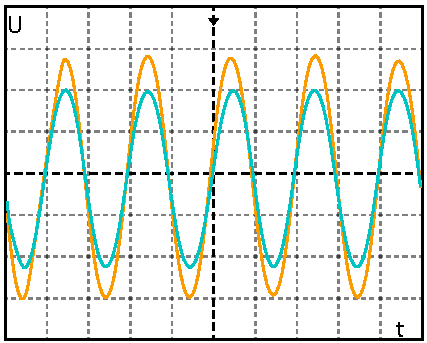
\includegraphics[width=0.9\linewidth]{7.pdf} \\  НМП}
\end{minipage}
\caption{Графііки $U_1$(поманчовий) та $U_2$ }
\label{ris1}
\end{figure}

\begin{figure}[h]
\center{\includegraphics[width=0.7\linewidth]{q.png}}
\caption{Амплiтудна характеристика НМП}
\end{figure}



\begin{figure}[h]
\center{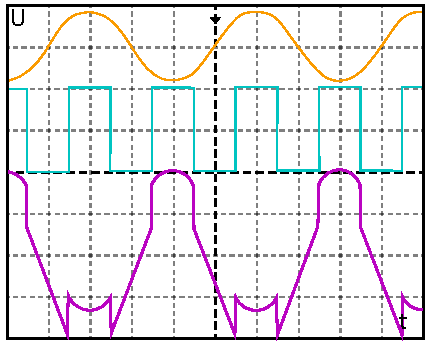
\includegraphics[width=0.6\linewidth]{14.pdf}}
\caption{Осцилограми $U_{11}(t)$, $U_{12}(t)$, $U_2(t)$ для ДМУ}
\end{figure}


\begin{figure}[h]
\center{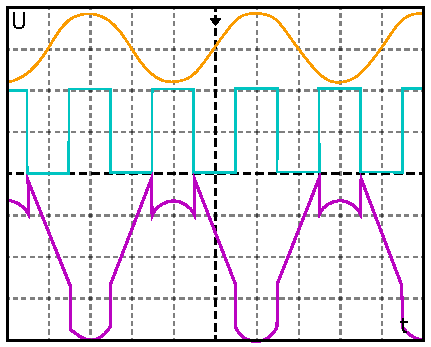
\includegraphics[width=0.6\linewidth]{15.pdf}}
\caption{Осцилограми $U_{11}(t)$, $U_{12}(t)$, $U_2(t)$ для ИСУ}
\end{figure}
\begin{figure}[h]
\center{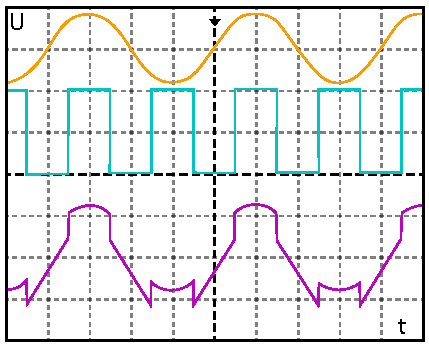
\includegraphics[width=0.6\linewidth]{16.pdf}}
\caption{Осцилограми $U_{11}(t)$, $U_{12}(t)$, $U_2(t)$ для НСУ}
\end{figure}

\clearpage
\newpage
\begin{center}Аналітичні вирази вихідної напруги для кожної схеми
\end{center}\par

IMП: $U_{\text {вих }}=-\dfrac{R_{3}}{R_{2}} \cdot U_{\text {ви}}$\\

HMП: $U_{\text {вих }}=\left(1+\dfrac{R_{3}}{R_{2}}\right) \cdot U_{\text {вх}}$\\

ICП: $U_{\text {вих }}=-\dfrac{R_{3}}{R_{1}} \cdot U_{11}-\dfrac{R_{3}}{R_{2}} \cdot U_{12}$\\

ДМП: $U_{\text {вих }}=-\dfrac{R_{3}}{R_{2}} \cdot U_{11}+\dfrac{R_{4}}{R_{1}+R_{4}} \cdot\left(1+\dfrac{R_{3}}{R_{2}}\right) \cdot U_{12}$\\

HCП: \\

$U_{\text {вих }}=\dfrac{R_{2}+R_{3}}{R_{2}} \cdot \dfrac{R_{4} R_{5}}{R_{4} R_{5}+R_{1} R_{5}+R_{1} R_{4}} \cdot U_{11}+\dfrac{R_{2}+R_{3}}{R_{2}} \cdot \dfrac{R_{4} R_{1}}{R_{4} R_{5}+R_{1} R_{5}+R_{1} R_{4}} \cdot U_{12}$\\

\begin{center}Підставляемо номінали резісторів
\end{center}\par

IMП: $U_{\text {вих }}=-\dfrac{20 \cdot 10^{3}}{10 \cdot 10^{3}} \cdot 100 \cdot 10^{-3}=-200 \text{ мВ}$\\

HMП: $U_{\text {вих }}=\left(1+\dfrac{20 \cdot 10^{3}}{10 \cdot 10^{3}}\right) \cdot 100 \cdot 10^{-3}=300 \text{ мВ}$\\

ICП: $U_{\text {вих }}=-\dfrac{20 \cdot 10^{3}}{10 \cdot 10^{3}} \cdot 100 \cdot 10^{-3}-\dfrac{20 \cdot 10^{3}}{10 \cdot 10^{3}} \cdot 100 \cdot 10^{-3}=-400 \text{ мВ}$\\

ДМП: $U_{\text {вих }}=-\dfrac{20 \cdot 10^{3}}{10 \cdot 10^{3}} \cdot 100 \cdot 10^{-3}+\dfrac{20 \cdot 10^{3}}{(10+20) \cdot 10^{3}} \cdot\left(1+\dfrac{20 \cdot 10^{3}}{10 \cdot 10^{3}}\right) \cdot 100 \cdot 10^{-3}=0$\\



НСП: \begin{align*}
U_{\text {вих }}=\dfrac{(10+20) \cdot 10^{3}}{10 \cdot 10^{3}} \cdot \dfrac{20 \cdot 10 \cdot 10^{6}}{20 \cdot 10 \cdot 10^{6}+10 \cdot 10 \cdot 10^{6}+20 \cdot 10 \cdot 10^{6}} \cdot 100 \cdot 10^{-3}+\\
+\dfrac{(10+20) \cdot 10^{3}}{10 \cdot 10^{3}} \cdot \dfrac{20 \cdot 10 \cdot 10^{6}}{20 \cdot 10 \cdot 10^{6}+10 \cdot 10 \cdot 10^{6}+20 \cdot 10 \cdot 10^{6}} \cdot 100 \cdot 10^{-3}=240 \text{ мВ}
\end{align*}





















\clearpage
\newpage
\begin{center}Висновки та оцінка результатів експерименту.\end{center}\par
В результаті проведеної цієї лабораторної роботи було виявлено певні особливості, які притаманні для ІМП та НМП, наприклад те що для схем з ІМП характерний менший вхідний опір ніж для НМП, а для обох схем зміна доданого опору на виході системи R4 майже не впливає на значення вихідного сигналу тому $\Rightarrow$ $R_{\text{вих}} = 0$. Для ІМП і НМП характерне відносно мале підсилення за напругою. Проте підсилення за струмом є більшим для НМП. Також можна стверджуват, що коефіцієнт підсилення инвертуючого каскаду ОП залежить тільки від параметрів зовнішнього ланцюга і не залежить від коефіцієнта посилення самого підсилювача.

\begin{figure}[h]
\center{\includegraphics[angle = -90, width=0.8\linewidth]{12345.jpg}}
\end{figure}




\end{document}
